%%%%%%%%%%%%%%%%%%%%%%%%%%%%%%%%%%%%%%%%%
% Journal Article
% LaTeX Template
% Version 1.3 (9/9/13)
%
% This template has been downloaded from:
% http://www.LaTeXTemplates.com
%
% Original author:
% Frits Wenneker (http://www.howtotex.com)
%
% License:
% CC BY-NC-SA 3.0 (http://creativecommons.org/licenses/by-nc-sa/3.0/)
%
%%%%%%%%%%%%%%%%%%%%%%%%%%%%%%%%%%%%%%%%%

%----------------------------------------------------------------------------------------
%	PACKAGES AND OTHER DOCUMENT CONFIGURATIONS
%----------------------------------------------------------------------------------------

\documentclass[twoside]{article}

\usepackage{lipsum} % Package to generate dummy text throughout this template
\usepackage{graphicx} % obrazky
\graphicspath{{images/}} % cesta k obrazkum
\usepackage[sc]{mathpazo} % Use the Palatino font
\usepackage[T1]{fontenc} % Use 8-bit encoding that has 256 glyphs
\linespread{1.05} % Line spacing - Palatino needs more space between lines
\usepackage{microtype} % Slightly tweak font spacing for aesthetics

\usepackage[hmarginratio=1:1,top=32mm,columnsep=20pt]{geometry} % Document margins
\usepackage{multicol} % Used for the two-column layout of the document
\usepackage[hang, small,labelfont=bf,up,textfont=it,up]{caption} % Custom captions under/above floats in tables or figures
\usepackage{booktabs} % Horizontal rules in tables
\usepackage{float} % Required for tables and figures in the multi-column environment - they need to be placed in specific locations with the [H] (e.g. \begin{table}[H])
\usepackage{hyperref} % For hyperlinks in the PDF

\usepackage{lettrine} % The lettrine is the first enlarged letter at the beginning of the text
\usepackage{paralist} % Used for the compactitem environment which makes bullet points with less space between them

\usepackage{abstract} % Allows abstract customization
\renewcommand{\abstractnamefont}{\normalfont\bfseries} % Set the "Abstract" text to bold
\renewcommand{\abstracttextfont}{\normalfont\small\itshape} % Set the abstract itself to small italic text

\usepackage{titlesec} % Allows customization of titles
\renewcommand\thesection{\Roman{section}} % Roman numerals for the sections
\renewcommand\thesubsection{\Roman{subsection}} % Roman numerals for subsections
\titleformat{\section}[block]{\large\scshape\centering}{\thesection.}{1em}{} % Change the look of the section titles
\titleformat{\subsection}[block]{\large}{\thesubsection.}{1em}{} % Change the look of the section titles

\usepackage{fancyhdr} % Headers and footers

%BIBLIOGRAFIE---------
\usepackage[backend=bibtex,sorting=none,bibstyle=ieee]{biblatex}
\addbibresource{bibliography.bib}


\fancyfoot[RO,LE]{\thepage} % Custom footer text

%----------------------------------------------------------------------------------------
%	TITLE SECTION
%----------------------------------------------------------------------------------------

\title{\vspace{-15mm}\fontsize{24pt}{10pt}\selectfont\textbf{Design and implementation of software for biomedical data analysis}} % Article title

\author{
\large
\textsc{Lukas Sulik}\\
\normalsize Faculty of Informatics and Management \\
\normalsize University of Hradec Kralove \\
\normalsize Hradec Kralove, Czech Republic \\
\normalsize \href{mailto:lukas.sulik@hotmail.com}{lukas.sulik@hotmail.com} % Your email address
\vspace{-5mm}
}
\date{}

%----------------------------------------------------------------------------------------

\begin{document}

\maketitle % Insert title



%----------------------------------------------------------------------------------------
%	ABSTRACT
%----------------------------------------------------------------------------------------

\begin{abstract}

\noindent Theoretical part of the article presents capsule endoscopy and its use in healthcare. Practical part is based on the development of a new program for capsule endoscopy and basic algorithms for detecting bleeding in the small intestine. The result is software based on the Java platform, using the OpenCV library and it can detect bleeding in the digestive tract.

\end{abstract}

%----------------------------------------------------------------------------------------
%	ARTICLE CONTENTS
%----------------------------------------------------------------------------------------

\begin{multicols}{2} % Two-column layout throughout the main article text

\section{INTRODUCTION}

The article deals with the analysis of biomedical data gathered from capsular endoscopy. Data are further processed using computer vision and processing software is searching for suspicious anomalies which could indicate the occurrence of the disease or bleeding.

The small intestine is the most difficult part of intestines to explore. It is because of the distance from the mouth and anus. And also because of its complicated shape, which may contain various loops. Conventional endoscopic techniques e.g. enteroscopy or colonoscopy are also limited by the length of the small intestine (3.35-7.85 m)\cite{randomized}.


Capsular endoscopy is based on a small camera having a size of a larger pill with own light source. The camera captures an images from the intestine and sends them wirelessly to a receiver located outside of the patient's body. The capsules battery can operate for 7- 8 hours. This time is sufficient in most cases for the examination of the entire small intestine \cite{diagnosing}. After completing the whole process, the camera is excluded through the digestive tract.

The gathered data is necessary to evaluate. It can only do a person with the required knowledge for this purpose. Due to the amount of records and their lengths it consumes a lot of time. However, there is opportunity to evaluate the data using special software that can detect potential diseases. Which may lead to shortening the process time for diagnosing the disease.

\begin{figure}[H]
	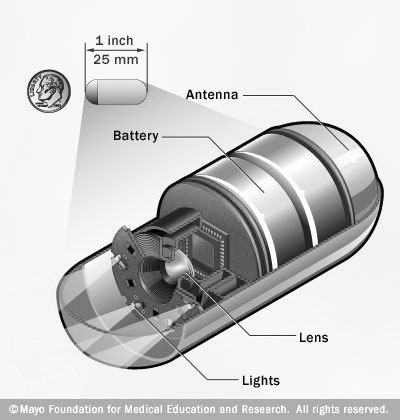
\includegraphics[scale=0.5]{capsule}
	\centering
	\caption{Capsule \cite{capsule} \label{fig:capsule}}
\end{figure}

%------------------------------------------------

\section{PROBLEM DEFINITION}
Developed application should be able to analyze record and detect possible bleeding in the intestines. Data are extracted from the camera to AVI format, but it is more closer to sequence of consecutive images than a smooth video. The problem arises in determining whether the blood is located in intestines.

It is necessary to describe or define the object, which we looking for. In that way that it will be possible to find it using computer vision techniques with as much accuracy is it possible and fewest errors. So we need to find EER between FAR and FRR as described in \ref{fig:eergraf}.

\begin{figure}[H]
	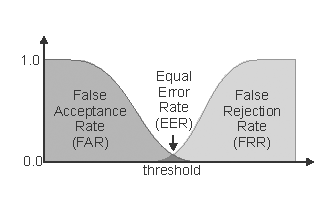
\includegraphics[scale=0.5]{eergraf}
	\centering
	\caption{EER graph \cite{gumption:}\label{fig:eergraf}}
\end{figure}

The biggest problem is the definition of the searched object, because the quality of the data is poor due to the low resolution  of cameras. There are also lots of anomalies in the data, which complicate the detection of the object (various reflections, food residues, similar colored spectrum ...). It will be necessary to combine multiple methods to achieve the best result.

\begin{figure}[H]
	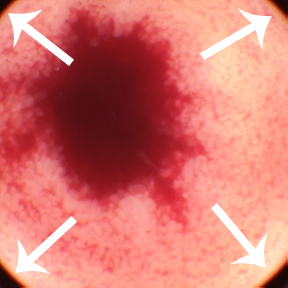
\includegraphics[scale=0.5]{anomalie}
	\centering
	\caption{Anomalies \label{fig:anomalie}}
\end{figure} 

In the article, "Detection of bleeding in wireless capsule endoscopy images using color range ratio" \cite{detection} authors deal with the possibility of detecting blood through the range of colors in the RGB model. This approach has many deficiencies in the real environment, because almost in every image can be located pixel in the same range, as defined blood range. According to the test they used two algorithms. Accuracy of first algorithm is only 48 \% and the second one is more accurate and have 98 \% accuracy.


Group of authors from the article "A technique for blood detection in wireless capsule endoscopy images" \cite{technique} used more sophisticated approach. They firstly filter image from unwanted objects which will eliminate some anomalies. And after that color range filter is used for determining blood. The results showed higher sensitivity and specificity of this approach and it leads to better results.

From the scientific articles is evident that they have quite good results on the selected database of samples. However the solutions are too focused on the detection according to color range which may lead to bad results in real environment.

\section{ALGORITHMS DESIGN}
It was not possible to use same approaches to detect all presence of blood in digestive tract. Thus two algorithms were developed. One for small stains of blood and second for large stains of blood. Both of them used almost same methods but different approaches. Only one part which is same for both algorithm is that at the beginning of image processing image is cropped because it may contain color anomalies on the edges of the sensor of the camera.

\subsection{Detection of small stains}
The algorithm is divided in two independent parts. They are compared after the execution and if there is a match between them then frame is positive.

The first part of algorithm is focused on filtering the image according to the specific color range, which is refined by other techniques.
\begin{enumerate}
	\item Converting color format from BGR to HSV. In HSV color space is possible to filter by color range more accurately, see fig. \ref{fig:alg_1}.E.
	\item Filter image matrix by defined color range. The result is a new matrix, which includes only selected colors and their values are represented as a binary data, there is a loss of the color information, see fig. \ref{fig:alg_1}.F.
	\item For all contiguous area, which are created from the previous step, calculates the area and retain only those which are larger than a certain value. This removes insignificant tiny areas that are probably caused by noise or other anomalies. And also discolored areas inside the contiguous areas are filled, see fig. \ref{fig:alg_1}.G.
	\item At all points with a value of 1 in the filtered matrix is copied from the HSV matrix color information, thereby returning the color information for further processing, see fig. \ref{fig:alg_1}.H.
	\item A morphological operation dilation according to the desired configuration is applied on the matrix. This will connect all the nearby points in the matrix and thus create larger contiguous area, which could potentially be blood, see fig. \ref{fig:alg_1}.I.
	\item For all contiguous areas after dilation is calculated bounding box and its cutted from the matrix.
	\item In each square is performed again filtering by color, but with a different "strictly" configuration. In the newly formed matrix only dilation is performed, not the filtering small artifacts. This has the effect that essentially no change or square disintegrated into multiple regions, or it is discard square from the potential detected areas.
	\item In each new square all contiguous area are found. They are framed by the bounding box and stored in the field which holds other rectangles of interest, see fig. \ref{fig:alg_1}.J.
\end{enumerate}

Second part of the algorithm is about detect edges and determine them as potential objects that are distinct from the background. The procedure is as follows:
\begin{enumerate}
	\item Converting color format from RGB to gray scale, since it is preferable to detect edges, see fig. \ref{fig:alg_1}.B.
	\item Gaussian blur by the defined configuration.
	\item Canny edge detection by the defined configuration, see fig. \ref{fig:alg_1}.C.
	\item For all continuous founded edges is calculated minimum enclosing circle. It serves as a simple approximation of finding object.
	\item Because there are a lot of anomalies when detecting edges especially, around the camera edges. Its necessary to remove these anomalies from the result. Its is done by removing these circles that their average is not exceeding the maximum defined average. Its almost impossible to remove some circle which should be count as positive, because this algorithm is only for detecting small stains of blood.
	\item Putting the potential positive matrices into auxiliary matrix, see fig. \ref{fig:alg_1}.D.
\end{enumerate}

As soon as they are available both parts of the algorithm, a matrix that contains the auxiliary circles and a list of rectangle of interest. That is evaluated whether the matrix is positive. This is done by iterating over all the squares in the list, and if there is any of square which have at least one point in the circle then frame is positive, see fig. \ref{fig:alg_1}.K.

\begin{figure}[H]
	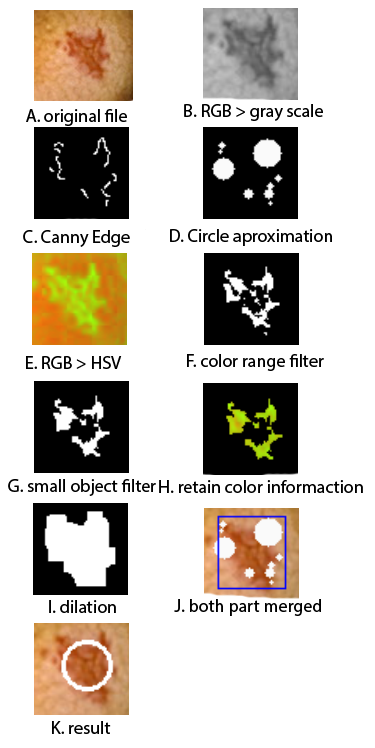
\includegraphics[scale=0.5]{alg1_clanek}
	\centering
	\caption{Example of detection of small stains algorithm. \label{fig:alg_1}}
\end{figure} 

\subsection{Detection of large stains}
The construction of a second algorithm is quite simpler and more straightforward than when detecting smaller stains. It is about finding a large area with the same color spectrum. The procedure is as follows:

\begin{enumerate}
	\item Converting color format from BGR to HSV. viz obr. \ref{fig:alg_2}.B.
	\item Filter image matrix by defined color range. viz obr. \ref{fig:alg_2}.C.
	\item Filter small particles. viz obr. \ref{fig:alg_2}.D.
	\item Morphological operation dilation, viz obr. \ref{fig:alg_2}.E.
	\item For all contiguous area in the matrix is measured their area. It is compared against a defined percentage of the total size of the area and if it is greater, frame is marked as positive. E.g. if the continuous area is larger than when 15 \% of the total area. viz obr. \ref{fig:alg_2}.F.
\end{enumerate} 

\begin{figure}[H]
	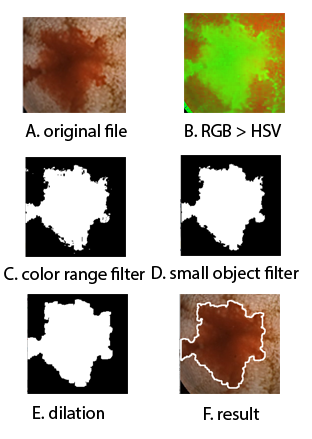
\includegraphics[scale=0.5]{alg2_clanek}
	\centering
	\caption{Example of detection of large stains algorithm. \label{fig:alg_2}}
\end{figure} 

\section{SOFTWARE IMPLEMENTATION}
The software is divided into four modules. Each module encapsulate specific functionality. Modules are Core, FXML, Application and Dev.

Module core is vital part of whole software. It contains almost all of the business logic. Encapsulate logic for loading algorithm, image processing, multitasking and generation of output files. Main packages of modul core are algorithm, video, task and output.

In package algorithm is functionality for loading initial configuration of algorithms and managing already loaded algorithms. The process of loading algorithm is made from few steps:
\begin{enumerate}
	\item Load all XML configuration files,.
	\item Using reflection find concrete algorithm class and make instance from it.
	\item Setup meta-data and initial configuration to instance from configuration file.
	\item Add new algorithm to the map.
\end{enumerate}

In the package video are only two classes VideoFrame and Buffer. Class VideoFrame is used to store information about a single video frame. Class has a matrix that represents the image, frame number and lock. Class buffer is server as a reservoir for video frames. It has self cleaning cycle for removing already processed video frames and has concurrent access for algorithms that are grabbing frames from the buffer.

Package task contains classes for asynchronous processing of the specific task. E.g task that grabbing data from the disk, task that running algorithms, task for buffer etc.

Last package is output. His mission is to create output files from result of the algorithms task. It can currently generate output file to PDF and XLSX. 

Module FXML is helper for manipulating JavaFX elements. It contains loader for custom fxml elements, abstract entry point to application, dialog facade and abstract controller.

Modul application is defined user interface for common users. It has dependency to module core and fxml. Application itself is based on design pattern model-view-control and contains only few helper classes and controllers, which are communicating with module core. There is no complicated logic.

Developing and debugging of algorithms is in module dev. It was created because author cannot find any suitable OpenCV developers tools for Java. It has only simple GUI, which is mostly generated by reflection from the algorithm configuration. It can show modification of algorithm configuration and his matrices in real time.

\section{TESTING OF DEVELOPED APPLICATION}

Testing and development of algorithm was primarily based on empirical research. Two samples were available for testing. First small sample of data were provided by Faculty hospital of Hradec Kralove. Sample is made from 21 pathological videos of various diseases and 16 video without any pathological occurrences. Each video file contains 201 frames. Data were extracted from cameras using their proprietary software and their quality were poor.

Second sample was obtained from the hospital after the development of algorithms and software. Second sample should prove the developed solution and algorithms within big data set. This sample lacks information from professionals about amount of pathological occurrences in the data set and due to amount of data author were able to determine it only approximately. Sample contained three full scan from real patients with pathological occurrence. Two of them were from PillCam and contained 23608 frames total and rest is from EndoCapsule with 87076 frames. This sample has better video quality because it was extracted with cooperation with Czech Academy of Science and their technologies to extract data from camera.

To measure effectiveness of algorithms are used standards in computer vision and biomedicine. Concrete used calculations are FRR (false rejection rate), FAR (false acceptance rate), SE (sensitivity) and SP (specificity).

\begin{table}[H]
	\centering
	\begin{tabular}{lllll}
		\toprule
		Name & FRR & FAR & SE & SP \\
		\midrule
		Positive & 2,95\% & 1,09\% & 78,36\% & 98,18\% \\
		Negative & 0,00\% & 0,83\% & N/A & 99,17\% \\
		\bottomrule
	\end{tabular}
	\caption{Average results of positive and negative video files}
	\label{tab:avgres}
\end{table}

Table \ref{tab:avgres} shows that the average sensitivity of the positive videos is 78.36 \%. It may seem a little, but due to the fact that the blood is in the intestines in various forms and shapes, and can not always determine all blood, since it is often very difficult. Most important thing to find is source of the bleeding or its biggest parts. Other undetected objects can be eg. blood mixed with liquids or very small particles around the edges.

Specificity and false acceptance rate are in all videos, with one exception, very good. It is possible to rapidly determine whether a patient is healthy or not. The exception is NOR1.avi video with 23.28 \% false positive images. It is due to that in video is a lot of reflections, which creates small anomalies.

False rejection rate is held within acceptable limits and images that contain blood are not rejected that much. An exception is sample from Endocapsule, because it contains massive bleeding. And it was already mentioned above, some of the images can not be accurately identified and it is essential to detect the source of bleeding. Unidentified object would probably not arise from something that could not be found and test would be depended on detection of side effects of bleeding.

Results of the performance and stability of software itself are satisfying. During the testing were detected some technical problems, especially in temporary storage of already detected anomalies for subsequent generating output files. Eg. in sample from Endocapsule it was detected 37889 frames as positive and it caused enormous memory requirements.

\section{CONCLUSIONS}
Developing of software was time consuming, but it was without any major problems. Author already had experiences with these technologies. Design of algorithms was more challenging, because author had only little experiences with computer vision. Invaluable help with algorithm design were consultations with Dr. Orcan Alpar.

Results of tests showed that the software is able to detect blood in the intestine with high accuracy. But for the more valuable results it's necessary to make further and more extensive tests on bigger data set or even better perform deployment into production environment.

The usability of solution lies in the simplifying work for people, who need to analyze the video files one by one, which is quite time consuming. It could be better to use their capacity elsewhere, where is not possible to use automated solutions.

%	REFERENCE LIST


\printbibliography

\end{multicols}

\end{document}
